\documentclass[11pt,a4paper]{article}
\usepackage[top=3cm, bottom=2cm, left=3cm, right=2cm]{geometry}
\usepackage[utf8]{inputenc}
% \usepackage[T1]{fontenc}
\usepackage{amsmath, amsfonts, amssymb}
\usepackage{siunitx}
\usepackage[brazil]{babel}
\usepackage{graphicx}
\usepackage[margin=10pt,font={small, it},labelfont=bf, textfont=it]{caption}
\usepackage[dvipsnames, svgnames]{xcolor}
\DeclareCaptionFont{MediumOrchid}{\color[svgnames]{MediumOrchid}}
\usepackage[pdftex]{hyperref}
\usepackage{natbib}
\bibliographystyle{plainnat}
\bibpunct{[}{]}{,}{s}{}{}
\usepackage{color}
\usepackage{footnote}
\usepackage{setspace}
\usepackage{booktabs}
\usepackage{multirow}
\usepackage{subfigure}
\usepackage{fancyhdr}
\usepackage{leading}
\usepackage{indentfirst}
\usepackage{wrapfig}
\usepackage{mdframed}
\usepackage{etoolbox}
\usepackage[version=4]{mhchem}
\usepackage{enumitem}
\usepackage{caption}
\usepackage{titlesec}




\titleformat{\section}{\LARGE\color{CarnationPink}}{\thesection}{1em}{}
\titleformat{\subsection}{\LARGE\color{CarnationPink}}{\thesubsection}{1em}{}


\DeclareCaptionLabelFormat{figuras}{\textcolor{CarnationPink}{Figura \arabic{figure}}}
\captionsetup[figure]{labelformat=figuras}

\makeatletter
\renewcommand\tagform@[1]{\maketag@@@{\color{CarnationPink}(#1)}}
\makeatother

\renewcommand{\theequation}{Eq. \arabic{equation}}
\renewcommand{\thefigure}{Fig. \arabic{figure}}
\renewcommand{\thesection}{\textcolor{CarnationPink}{\arabic{section}}}

\setlist[itemize]{label=\textcolor{CarnationPink}{$\mathbf{\square}$}}

\setlist[enumerate]{label=\textcolor{CarnationPink}{\arabic*.}, align=left}


\newcounter{exemplo}

\NewDocumentEnvironment{exemplo}{ O{} }{%
\allowbreak
\setlength{\parindent}{0pt}
  \begin{mdframed}[
  leftline=true,
  topline=false,
  rightline=false,
  bottomline=false,
  linewidth=2pt,
  linecolor=CarnationPink,
  frametitlerule=false,
  frametitlefont=\Large\bfseries\color{CarnationPink},
  frametitle={\color{CarnationPink}\normalfont\bfseries #1},
  ]
}{%
  \end{mdframed}
}

\setlength{\fboxsep}{5pt}
\setlength{\fboxrule}{1.5pt}
\usepackage{float}
\renewcommand{\thefootnote}{\alph{footnote}}
\usepackage{url}
\hypersetup{
	colorlinks=true,
	linkcolor=DarkTurquoise,
	filecolor=DarkTurquoise,      
	urlcolor=DarkTurquoise,
	citecolor=DarkTurquoise,
	pdftitle={Radioterapia}
}
\pagestyle{fancy}
\fancyhf{}
\renewcommand{\headrulewidth}{0pt}
\rfoot{Página \thepage}

\title{Resumo}
\author{Notas Rápidas \nocite{*}}
\date{\textit{Dalila Mendonça}}
\begin{document}
	\maketitle
    
\begin{exemplo}[5. Tratamentos com Fótons]
    \textcolor{CarnationPink}{Qualidade Do Feixe}
    \begin{itemize}
        \item A qualidade do feixe descreve o espectro de energia de um feixe de fótons de raios X (ou raios gama). Alguns feixes de fótons, por exemplo, \ce{^{60}Co}, são quase monoenergéticos (média de 1,25 MeV). Outros feixes, por exemplo, um feixe linac de 6 MV, são polienergéticos. MeV implica uma energia, enquanto 6 MV implica um espectro, com 6 MeV como a energia máxima. A qualidade do feixe de cada fabricante e cada máquina é ligeiramente diferente para feixes com a mesma energia nominal. Para feixes de fótons utilizados em radioterapia, a qualidade do feixe é medida por uma curva chamada curva de Porcentagem de dose na profundidade (PDP). A razão entre o valor da PDP a 20 cm e o valor da PDP a 10 cm de profundidade é freqüentemente utilizado para determinar a qualidade do feixe através de um valor. Para feixes de diagnóstico, o kVp ou camada semi-redutora é usada para definir a qualidade do feixe em vez da PDP;
        
        \item O endurecimento do feixe ocorre quando o feixe passa por qualquer material, que atua como um filtro, absorvendo os fótons de baixa energia. O feixe transmitido terá uma energia média aumentada e uma taxa de dose diminuída enquanto a energia máxima permanece inalterada. Para um feixe de diagnóstico, esse aumento na energia resulta em um aumento na HVL. Na figura, o espectro preto é o feixe inicial e o cinza é o feixe filtrado.

        \begin{center}
            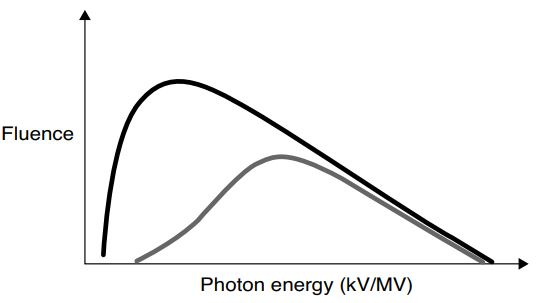
\includegraphics[width=0.5\textwidth]{Imagens/endurecimentoDoFeixe.JPG}
        \end{center}

        \item O output em um tubo de raios X kV é proporcional à corrente do tubo, porporcional ao quadrado da tensão do tubo e exponencialmente proporcional à corrente do filamento.
        
        \item O Cerrobend utilizado na confecção dos blocos em radioterapia é uma liga de bismuto, chumbo, estanho e cádmio. É útil como um material de alta densidade (\qty{9.4}{g/cm^3} ) e alto Z com um baixo ponto de fusão para criar rapidamente um bloco na forma desejada. O objetivo é atingir menos de 5\% de transmissão do feixe primário, o que significa 4.3 camadas semi-redutoras de cerrobend ou mais. 
        
        \item Um filtro físico também chamado de filtro em cunha, é formado por um material metálico com formatro triangular que gera um gradiente de intensidades do feixe na profundidade. Isso filtra diferencialmente os raios X de baixa energia, levando ao endurecimento do feixe. O grau de endurecimento do feixe é mais pronunciado perto do “calcanhar” mais grosso do filtro. Um filtro físico também é responsável pelo aumento do espalhamento da radiação.
        
        \item Um filtro virtual não produz endurecimento de feixe variável, pois o perfil de gradiente é criado pela abertura lenta de uma mandíbula do colimador do acelerador linear, em vez da transmissão através de Um filtro físico. Qualquer espalhamento pela mandíbula é reduzido pela blindagem no cabeçote da máquina e não contribui significativamente para a dose recebida pelo paciente.
        
        \item Quanto a distribuição espacial dos fótons produzidos por bremsstrahlung, para energias de elétrons incidentes na ordem de kV, os raios X são produzidos isotropicamente (em todas as direções). Com energias de elétrons incidentes da ordem de megavolt (MV), a distribuição de raios-X torna-se progressivamente mais alinhada com a direção dos elétrons incidentes. Portanto, um tubo de raios-X kV pode usar um alvo de reflexão onde os raios-X úteis estão a 90° do feixe de elétrons, enquanto um acelerador linear MV usa um alvo de transmissão onde os raios-x úteis serão emitidos aproximadamente na direção da velocidade dos elétros que incidem o alvo.

        \item Um filtro Thoraeus é comumente usado com tubos de raios-X de diagnóstico. O filtro consiste em camadas de estanho, cobre e alumínio para remover fótons de baixa energia e raios X característicos do feixe primário. Esses fótons de baixa energia não contribuem para a qualidade da imagem, mas aumentam a dose do paciente.
        
        \item A ordem das camadas do filtro Thoraeus é importante porque o estanho é o que mais contribui para a filtração dos raios X característicos do alvo de tungstênio, que ficam entre 58 keV e 69 keV. Os raios X característicos do estanho são de energia muito baixa e podem ser filtrados com cobre. Os raios X característicos do cobre são filtrados por uma fina película de alumínio, levando a um feixe endurecido capaz de produzir imagens nítidas.
        
        \item As interações de Bremsstrahlung ocorrem quando um elétron de alta energia passa perto do núcleo de um átomo. O elétron é desviado de sua trajetória original pelo núcleo devido à sua força coulombiana. O elétron sofre aceleração repentina em uma direção diferente (desacelerado), fazendo com que o elétron perca toda ou parte de sua energia nesse processo, que é convertida em um fóton. Um único elétron pode passar por múltiplas interações de bremsstrahlung antes de finalmente parar.
        
        \item Feixes de fótons de alta energia são criados por interações bremsstrahlung e, portanto, contêm um espectro de energia. A energia mais provável é aproximadamente um terço da energia máxima, que por convenção é usada para nomear o feixe (Energia nominal). Portanto, para um feixe de 10 MV a energia máxima é de 10 MeV e a energia mais provável é de aproximadamente 3,33 MeV. Isso não é o mesmo que a energia média, que é mais difícil de calcular.
        
        \item A filtração inerente em um acelerador linear é normalmente causada pelo próprio alvo de tungstênio (conforme os elétrons interagem com o alvo, um espectro de fótons é criado por meio de interações bremsstrahlung). Os fótons de baixa energia produzidos podem interagir e ser absorvidos pelo tungstênio remanescente antes de emergir para fora do alvo como parte do espectro. Este efeito aumenta à medida que a espessura do alvo aumenta. 
        
        \item A filtragem adicional é intencionalmente colocada no caminho de um feixe com o objetivo de aumentar a energia média do feixe (causando o endurecimento do feixe) ou diminuir a intensidade de um feixe.
        
        \item A penumbra do feixe (umbra é latim para “sombra”) é a redução gradual da intensidade do feixe na borda de um campo de fótons. É tipicamente medido como a largura entre as linhas de isodose de 80\% e 20\%, embora também sejam usadas linhas de isodose de 90\% a 10\%.
        
        \item Existem três fontes principais de penumbra do feixe que são a penumbra de transmissão, a penumbra geométrica e a penumbra interna. A penumbra de transmissão ocorre quando o feixe passa pela borda dos jaws, blocos ou colimadores multilâminas (MLC). A penumbra geométrica ocorre porque a fonte não é uma fonte pontual. A penumbra interna ocorre devido ao espalhamento dentro do paciente.
        
        \item O Cobalto-60 gera um feixe quase monoenergético (1,17 MeV, 1,32 MeV combinados para uma média de 1,25 MeV) e, portanto, o HVL1 = HVL2 = HVL3. No entanto, os tubos de diagnóstico usam a geração de raios-X bremsstrahlung para produzir um espectro de energias. Depois que o feixe passa pelo primeiro HVL, devido ao conceito de “endurecimento do feixe”, o segundo HVL agora é maior que o primeiro.
        
        \item A intensidade dos raios-X tem um pico direto (forward peaked) após o alvo e antes do filtro aplanador. O filtro aplanador é mais espesso no meio e afunila em direção às bordas, de modo que a região central seja atenue mais o feixe do que a periferia do filtro para tornar o feixe plano em uma profundidade específica. Como resultado, o feixe será mais endurecida no centro do que na periferia (menor energia média na periferia). Isso resulta em um feixe que atinge profundidades superiores a 10 cm. O filtro aplanador também reduz significativamente a taxa de dose.
        
        \item O feixe plano é especificado a 10 cm de profundidade e dentro da área delimitada por 80\% do tamanho do campo ou 1 cm dentro da borda do campo. A planicidade do feixe deve estar dentro de +–3\% da dose do eixo central a 10 cm de profundidade.
        
        \item Um filtro inclina as linhas de isodose em direção à sua borda fina. O ângulo entre o eixo central e as linhas de isodose a 10 cm de profundidade é o ângulo do filtro.
        
            \begin{center}
                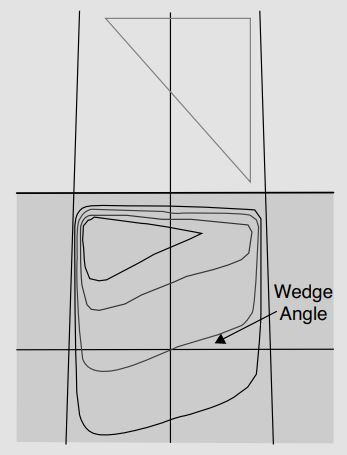
\includegraphics[width=0.5\textwidth]{Imagens/distruibuicaoDoseFiltro.JPG}
            \end{center}

        \item Feixes opostos paralelos são freqüentemente usados em radioterapia. Eles fornecem distribuição de dose uniforme para o alvo com uma configuração simples e reprodutível. Uma desvantagem dessa técnica é chamada de “efeito lateral do tecido”. O ponto médio entre os feixes opostos é o ponto de prescrição. A relação entre a dose máxima e a dose do ponto médio (ponto de prescrição) aumenta com a espessura do paciente e diminui com a energia. Como resultado, é melhor usar feixes de raios X de maior energia (>10 MV) para pacientes grandes (>20 cm) para melhorar a homogeneidade da distribuição da dose e preservar o tecido subcutâneo.
        
        \item A dose integral é simplesmente massa x dose se a dose for uniforme em toda a região, ou a soma da energia depositada. Se for calculado o histograma de volume de dose, a dose integral é a área sob o contorno externo, que inclui todo o tecido do paciente. A unidade de “dose integral” é kg/Gy ou joule. É usado para determinar a qualidade do plano de tratamento em relação à quantidade de dose administrada fora do alvo. A dose integral diminui com a energia.
        
        \item Novos aceleradores lineares (linacs) estão disponíveis com feixes FFF. Os Linacs requerem um filtro aplanador para produzir feixes planos em grandes campos abertos. No entanto, o filtro aplanador reduz a taxa de dose da máquina e produz o endurecimento do feixe. Com tratamentos de radioterapia com intensidade modulada (IMRT) para campos pequenos , os colimadores multilâminas (MLCs) são usados para modular deliberadamente a intensidade do feixe. Para esses tratamentos, o filtro não é mais necessário. As vantagens dessa abordagem incluem uma taxa de dose significativamente aumentada (>1.000 MU/min versus 300 a 600 MU/min) e e diminuição da variação no espectro de energia produzido(que é maior para feixes plano devido ao endurecimento do feixe). As desvantagens dessa abordagem incluem um possível aumento na dose da pele (menor endurecimento do feixe aumentando a quantidade de fótons de baixa energia) e a incapacidade de tratar campos grandes, planos e abertos sem o uso de MLCs. Alguns fabricantes adicionam um filtro fino para remover fótons de energia muito baixa para feixes não planos.
        
        \item A “energia efetiva” é definida como a energia de um feixe de raios X monoenergético que tem a mesma camada semi-redutora que o feixe heterogêneo de raios X.
        
        \item O valor da Porcentagem de dose na profundidade (PDP) a 10 cm de profundidade para um tamanho de campo de 10 cm x 10 cm com distância da fonte à pele de 100 cm é usado para definir a qualidade do feixe.
        
        \item Diferentemente dos fótons, as energias dos elétrons são escritas como megaelétrons volts (MeVs) porque as energias de elétrons são monoenergéticas quando deixam o guia de ondas acelerado, mas os fótons apresentam um feixe polienergético. A energia do fóton MV representa o raio-X de maior energia (em MeVs) no espectro.

    \end{itemize}

    \textcolor{CarnationPink}{Fatores que Afetam a deposição de dose pelos fótons}
    \begin{itemize}
        \item Para um determinado tamanho de campo, a PDP (expressa em porcentagem) é medida ao longo do eixo central e é definida como a razão de uma dose em uma determinada profundidade d para a dose em uma profundidade de referência (geralmente d\textsubscript{max}) no eixo central.
        
            $$PDP = \frac{Dose\;na\;profundidade\;d}{Dose\;na\;profundidade\;de\;referencia\;d_{max}} \times 100\%$$

            $$PDP(d) = \frac{D(d)}{D(d_{max})} \times 100\%$$

        \item A PDP em uma produndidade d pode ser afetada por variaçoes no tamanho de campo, energia, SSD e pela utilização de filtros da seguinte maneira:
        
            \begin{enumerate}[label=\roman*)]
                \item Com o aumento do tamanho de campo, a PDP(d) irá aumentar devido ao aumento do espalhamento no meio.
                \item Cpm Aumento da energia do feixe, a PDP(d) irá aumentar devido ao aumento da penetração;
                \item Com o Aumento da SSD a PDP(d) irá aumentar devido à lei do inverso quadrado, pois a dose em $d_{max}$ irá diminuir.
                \item Com a inserção de um filtro físico ocorrer o endurecimento do feixe e portanto ocorrerá um aumento na PDP. 
            \end{enumerate}

        \item A curva de PDP relata a deposição de dose em função da profundidade de um feixe de radiação. O PDP na superfície para energias de megavoltagem está abaixo de 100\%, pois os fótons incidentes produzem elétrons de alta energia que percorrem uma distância antes de parar e depositar energia. Este efeito explica as propriedades de “skin sparing” da terapia de megavoltagem. O pico na curva conhecida como D\textsubscript{max}, ocorre em uma maior profundidade. A curva então declina, ou atenua, devido a uma combinação da lei do inverso do quadrado, absorção e espalhamento.
        
        \begin{center}
            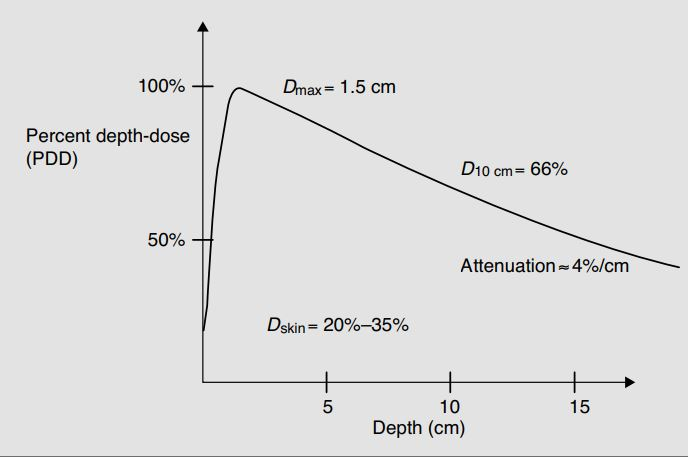
\includegraphics[width=0.5\textwidth]{Imagens/pdp.JPG}
        \end{center}

        \item Os valores de d\textsubscript{max} são sutilmente diferentes para cada máquina e feixe, porém os valores tipicos para cada energia nominal são:
        
            \begin{enumerate}[label=\alph*)]
                \item \ce{^{60}Co}: 0.5 cm;
                \item 6 MV: 1.5 cm;
                \item 10 MV: 2.5 cm;
                \item 15 MV: 3.0 cm;
                \item 18 MV: 3.2 cm até 3.5 cm
            \end{enumerate}

        \item Sob as condições de referência, um feixe de \ce{^{60}Co} atenua aproximadamente 4\% por cm.  Feixes de Fótons de 6 MV atenuam aproximadamente 3.5\% por centímetro. E Feixes de 10 MV atenuam aproximadamente 3.3\% por centímetro. Esses valores são uma aproximação, pois os valores de atenuação mudam com a produndidade.
        
        \item Normalmente, os valores de PDP ou TMR são tabelados apenas para campos quadrados. Um campo retangular terá aproximadamente a mesma PDP ou TMR que seu campo quadrado equivalente. Existem também outros métodos mais complexos para aproximar a PDD ou a TMR para formas de campo irregulares, como o método de Clarkson.
        
        \item A PDP é normalmente determinada para valores de SSD de 100 cm. Para estimar a PDP para diferentes valores de SSD é utilizado o Fator de Mayneord (F). o Fator F é uma estimativa das mudanças na PDP causadas apenas pela lei do inverso quadrado. Este fator assume que a quantidade de espalhamento é constante a medida que a SSD muda, o que não é correto e portanto limita a precisão deste método. Para baixas energias, a correção da razão tecido-ar (TAR) para o método do fator Mayneord F pode ser usada se as tabelas TAR estiverem disponíveis.
        
        \item O tamanho do campo é normalmente definido no isocentro da máquina, a 100 cm da fonte. Isso seria, então, na superfície do paciente para a configuração da distância da fonte à pele (SSD) ou no isocentro para a configuração da distância da fonte ao eixo (SAD).
        
        \item Fotons com energias superiores a 10 MV não são recomendados para o tratamento de câncer de pulmão. A diferença na densidade eletrônica entre o pulmão e o tecido mole ou osso da parede torácica apresenta problemas especiais no manejo do câncer de pulmão. Fótons de alta energia podem contribuir para aumentar a dose espalhada no pulmão. Além disso, a maior região de build-up para fótons de alta energia pode comprometer a cobertura do tumor em sua periferia.
        
        \item A região de buildup é a região inicial na curva de PDP, entre a superfície do paciente e d\textsubscript{max}. A deposição de dose pelos fótons depende de elétrons secundários. Enquanto os fótons são constantemente atenuados exponencialmente em função da lei do quadrado inverso, os fótons de alta energia requerem alguma profundidade no tecido para gerar elétrons secundários, explicando assim porque a dose depositada é baixa na superfície do tecido irradiado.
        
        \item A profundidade de d\textsubscript{max} diminui ligeiramente em função do tamanho do campo. Por exemplo, um d\textsubscript{max} de 1,5 cm é estimado para um fóton de 6 MV e um campo de 10 cm x 10 cm, enquanto para um campo de 20 cm x 20 cm esperasse uma  d\textsubscript{max} de 1,4 cm. Isso se deve ao aumento do espalhamento que contribui para a deposição superficial da dose, aproximando d\textsubscript{max} da superfície.
        
        \item A PDP aumenta à medida que o tamanho do campo aumenta devido ao espalhamento no tecido fora do eixo central (off-axis). Tanto a dose primária (fótons emitidos diretamente do cabeçote do linac) quanto a dose secundária (espalhamento no tecido) contribuem para a PDP. Embora tanto a dose na profundidade d (D\textsubscript{d}) quanto a dose em d\textsubscript{max} aumentam, o D\textsubscript{d} aumenta mais que a dose em d\textsubscript{max}(D\textsubscript{max}), portanto a PDP aumenta.
        
        \item O aumento da PDP com o tamanho de campo é maior para feixes de baixa energia. Com altas energias, a maior parte do espalhamento ocorre na mesma direção do fóton incidentee portanto o espalhamento lateral é menor.
        
        \item As maiores vantagens em se utilizar a técnica SAD (que utiliza o fator TMR) quando comparado a técnica de SSD (que utiliza o fator PDP) é que os cálculos utilizando a PDP são convenientes quando não há mudanças na SSD e a SSD é mantida na distância padrão de calibração igual a 100 cm. No entando, um tratamento com diversos campos, a SSD irá mudar devido a variações na superfície do paciente, ou então o paciente deverá ser movido em todo campo de tratamento para igualar a SSD à SSD de calibração. Ao utilizar o método de SAD, utiliza-se a TMR ao invés da PDP, e como a TMR é independente da SSD, torna-se uma vantagem nessas situações de SSD variáveis. 
        
        \item A Razão Tecido-AR (TAR - tissue-to-air ratio) é definida como a dose em um ponto no tecido dividida pela dose no ar no ponto com a mesma distancia à fonte. Devido a distância até a fonte para ambas componentes da razão serem as mesmas, a TAR não varia com a SSD, fornecendo uma vantagem para cálculos com a SSD variável (vários campos com setup SAD). Se o campo aumenta, mantendo a profundidade constante, haverá mais espalhamento no tecido, e portando o termo do numerador irá aumentar. No entanto, não há espalhamento no ar e o denominador se mantém constante, levando a um aumento na TAR. Uma vez que altas energias são mais penetrantes no tecido, a TAR aumenta com o aumento na energia.

            \begin{center}
                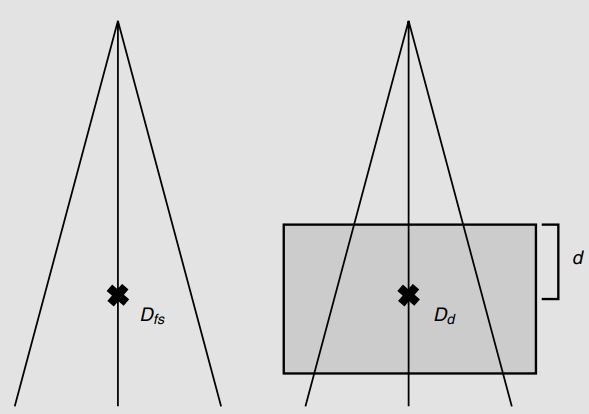
\includegraphics[width=0.5\textwidth]{Imagens/tar.JPG}
            \end{center}
        
        \item O diagrama abaixo mostra a relação entre a Porcentagem de Dose na profundidade (PDP) a  Razão Tecido-Ar (TAR) a Lei do Inverso Quadrado (ISL) e o fator de espalhamento de pico (PSF) que é definido como a TAR na produndidade de dose máxima d\textsubscript{max}:
        
            \begin{center}
                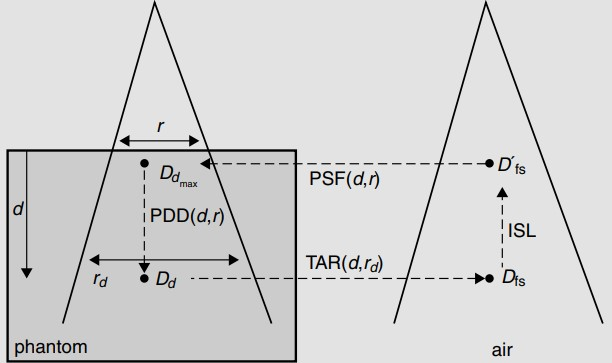
\includegraphics[width=0.5\textwidth]{Imagens/relacoes.jpg}
            \end{center}        
            
            $$D_d = \frac{PDP(SSD, D, r) \times D_{max}}{100}$$

            $$D_{fs} = \frac{D_d}{TAR(d, r_d)}$$

            $$D_{fs}' = \sqrt{D_{fs}^2\left(\frac{SSD}{SSD + d}\right)^2}$$

            
            $$D_{d_{max}} = PSF(r) \times D_{fs}'$$
        
        \item O fator BSF (backscatter factor) é um caso especial da PSF (peak scatter factor) quando fótons de baixa energia com um d\textsubscript{max} igual a zero são considerados. Se d\textsubscript{max} é perto de zero, o único espalhamento que contribui para dose em d\textsubscript{max} é devido ao retroespalhamento, e por isso o nome ``backscatter''. 


        \item Uma vez que os fótons de alta energia tendem a espalhar ``para frente'' o PSF diminui em apenas poucos por cento para feixes de alta energia (PSF varia de 1.05 até 1.1). O PSF, ou mais precisamente, o fator de retroespalhamento é maior para fótons de baixa energia devido ao aumento do espalhamento lateral no tecido (pode ser mais alto em aproximadamente  40\% a 50\% para feixes de diagnóstico).
        
        \item A TMR é dada pela equação:
        
            $$TMR(d) = \frac{D(d, SAD)}{D(d_{max}, SAD)}$$

            Neste caso as doses são calculadas nas profundidades d e $d_{max}$ e ambas possuem a mesma distância até a fonte (portando o ponto deve ser posicionado na distância de referencia)
        
            \begin{center}
                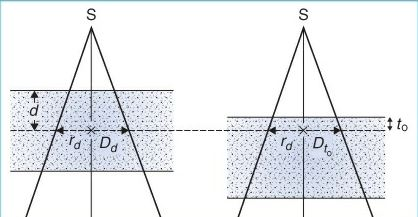
\includegraphics[width=0.5\textwidth]{Imagens/tmr}
            \end{center}

        \item A TMR está relacionada com a TAR a partir do PSF:
        
            $$TMR = \frac{TAR}{PSF}$$

        \item A diferença entre a PDP e a TMR é que, embora ambas sejam dadas pela razão entre a dose no ponto e a dose na profundidade máxima, A PDP é calculada utilizando a mesma Distância da Fonte até a Superfície (SSD) em profundidades diferentes enquanto que o TMR é calculado utilizando a mesma distância da fonte ao eixo (SAD) e portanto é independente da SSD. 
        
        \item Em pacientes que irão tratar regiões onde á irregularidades na superfície da pele,; uim bolus pode ser colocado na superfície da pele para uniformizar a irregularidade da superfície do paciente. A adição de um bolus removerá, no entanto, o efeito poupador da pele da radiação de megavoltagem. Alternativamente, filtros compensadores podem ser usados. Um filtro compensador atenua o feixe na região do “tecido ausente”. Outras técnicas para controlar as irregularidades da superfície incluem o uso de filtros em cunha ou o blindagem de partes do tecido em algumas das frações do tratamento.
        
        \item O tamanho de campo é definido pela linha de isodose de 50\%. O tamanho de campo muda com a distância devido a divergencia do feixe e então é definido no isocenteo da máquina.
        
        \item O método de Clarkson é utilizado para calcular a dose para campos irregulares. Esta técnica envolve dividir um campo irregular em diversas regiões para aproximar o espalhamento para cada região. 
    \end{itemize}

    \textcolor{CarnationPink}{Cálculo de Unidades Monitoras}
    \begin{itemize}
        \item As condições de referência são as condições nas quais o feixe é calibrado. É extremamente importante especificar essas condições, caso contrário, podem ocorrer erros sistemáticos nos cálculos de dose. Um exemplo de condições de referência comuns é que o feixe pode ser calibrado (de acordo com AAPM TG-51) de modo que 1 unidade monitora (1 MU) seja igual a dose de 1 cGy depositada por um fóton de 6 MV na profundidade d\textsubscript{max} usando um tamanho de campo de 10 cm x 10 cm em água com uma distância da fonte à superficie (SSD) de 100 cm. Observe que o tamanho do campo é determinado a 100 cm da fonte.
        
        \item A dose em um ponto na profundidade é dada pela soma da dose devido à radiação primária (proveniente do feixe primário emitido pelo acelerador) e a dose espalhada proveniente do espalhamento dentro da máquina ou dentro do paciente.
        
        \item $S_c$ é o fator de espalhamento do colimador e $S_p$ o fator de espalhamento do phantom (tecido). Os fótons que interagem com objetos presentes no cabeçote do acelerador, como o alvo, o filtro aplanador, os jaws colimadores, tendem a se espalhar e entrar no paciente em vários ângulos (Sc). Uma vez que os fótons entram no paciente, eles são espalhados novamente (Sp). Sc e Sp são principalmente uma função do tamanho de campo, uma vez que mais espalhamento ocorre em aberturas de campo maiores. Como são fatores de correção, eles são tipicamente próximos de 1, mas podem variar de 0,9 para campos pequenos a 1,1 para campos grandes. Às vezes, para simplificar, eles são combinados em um único termo, $S_{c,p}$, que é simplesmente Sc x Sp. Observe que o tamanho do campo para $S_c$ é definido no isocentro. No entanto, o tamanho do campo para $S_{p}$ é definido na profundidade, uma vez que o espalhamento interno pode mudar à medida que o feixe diverge com a profundidade.
        
        \item O fator $S_c$ é definido como a razão entre o output para um dado tamanho de campo e o output para o campo de referência (10 cm x 10 cm) ambos medidos no ar no isocentro (100 cm). Esta medida é feita com uma câmara de ionização com uma capa de build-up.
        
        \item o fator $S_p$ é a razão entre a taxa de dose para um determinado tamanho de campo e a taxa de dose  para o tamanho de campo de referência (10 cm x 10 cm) medida em um phantom na profundidade $d_{max}$ ou profundidade de referência com abertura de colimador idêntica. Teoricamente, poderia ser medido usando fantomas de vários tamanhos com uma abertura de colimador maior. Mas, na prática, é medido indiretamente usando a seguinte equação:
        
            $$S_p(r) = \frac{S_{c,p}(r)}{S_c(r)}$$

        onde $S_{c,p}(r)$ é o fator de espalhamento total definido como a taxa de dose na profundidade de referência para um dado tamanho de campo r dividido pela taxa de dose no mesmo ponto e profundidade para o campo de referência. o $S_{c,p}(r)$ normalmente é medido em profundidades de referência maior que $d_{max}$ para evitar a contaminação com eletrons e então é convertido para $d_{max}$ através da PDP.

        \item De acordo com o TG-71, o cálculo de MU para o setup SSD simplificado (sem considerar Fator Off-axis, fator filtro e demais modificadores de feixe) é dado através da seguinte equação:
        
            $$MU = \frac{D}{D_0' \cdot S_c(r_c) \cdot S_p(r_{d}) \cdot PDP_N(d, r, SSD) \cdot \left(\frac{SSD_0 + d_0}{SSD + d_0}\right)^2}$$

            \begin{itemize}[label=\textopenbullet]
                \item $D$: A dose no ponto de interesse.
                \item $D_0'$: Dose por UM em condições de calibração.
                \item $d$: Profundidade do ponto de cálculo.
                \item $d_0$: A profundidade de normalização para dosimetria de fótons e elétrons, normalmente $d_{max}$.
                \item $r_c$: O lado do quadrado equivalente para o tamanho do campo do colimador definido no isocentro.
                \item $r_d$: O lado do quadrado equivalente para o tamanho do campo incidente no paciente, definido na superfície e na profundidade d, respectivamente.
                \item $S_c$: Fator de dispersão do colimador.
                \item $S_p$: fator de dispersão do phantom 
                \item $PDP_N$: é a PDP / 100.
            \end{itemize}

        \item De Acordo com o TG-71, o cálculo de MU para o setup SAD é dado por:
        
            $$MU = \frac{D}{D_0' \cdot S_c(r_c) \cdot S_p(r_{d}) \cdot TPR(d, r_d) \cdot WF(d, r_d, x) \cdot TF \cdot OAR(d, x) \cdot \left(\frac{SSD_0 + d_0}{SPD}\right)^2}$$

            \begin{itemize}[label=\textopenbullet]
                \item $SPD$: é a distancia do ponto até a fonte;
                \item $TPR$: é a razão tecido máximo;
                \item $TF$: é o fator de transmissão;
                \item $WF(d, r_d, x)$: é o fator filtro na produndidade d a uma distância x do eixo central;
                \item $OAR(d, x)$: é o fator off-axis para uma distância x do eixo central.
            \end{itemize}

        \item Uma “regra de ouro” é que o cobalto-60 decai aproximadamente 1\% ao mês. Embora esta seja uma boa resposta a ser lembrada para estimativa, ela não funcionará por um longo período de tempo. A resposta precisa, é utilizando a lei de decaimento exponencial com o tempo de meia vida de 5.26 anos e o tempo de análise igual a 1 mês. 
        
        \item As máquinas de Cobalto-60 apresentam maior penumbra geométrica devido a fonte de cobalto ser normalmente um cilindro com diâmetro variando entre 1cm a 2cm, diferentemente do diâmetro do feixe estreito de elétrons utilizado nos aceleradores lineares que possui diâmetro de aproximadamente 3 mm ao interagir com o alvo de tungstênio.
        
        \item Os equipamentos de Cobalto-60 são controlados através de um timer. Devido a fonte estar sempre ``ligada'', pois se trata de um material radioativo, a fonte é sempre mantida dentro de uma blindagem no cabeçote da máquina e a blindagem só é removida no momento em que o paciente está sendo tratado. A calibração de uma bomba de cobalto é ralizada então atraves da medida do tempo que leva para uma fonte depositar sua dose, no qual é uma função da atividade da fonte. Uma fonte mais nova tem tipicamente uma taxa de dose de 240cGy/min na SAD de 80 cm.

        \item A correção de tempo em tratamentos com cobalto-60 leva em conta o tempo que leva para afastar a blindagem da fonte de cobalto. Por uma fração desse tempo, a fonte não está totalmente exposta e não está fornecendo a taxa de dose total. Portanto, o erro de tempo é adicionado ao tempo que leva para entregar a fonte.

    \end{itemize}
\end{exemplo}

\begin{exemplo}[6. Básico de Planejamento de Tratamento]
    \begin{itemize}
        \item Em um tratamento de crânio total (WB) normalmente são utilizados dois campos laterais deslocados \ang{5} para a direção anterior do paciente, resultando em um campo com angulação de \ang{275} e um campo com angulação de \ang{85}. Este deslocamento no ângulo do gantry é feito para evitar a divergência do feixe nos cristalinos, minimizando a dose depositada nessas estruturas. 
        
        \item O belly board é um acessório de imobilização comumente utilizado em tratamentos de cancer retal. O belly board consiste em um ``colchão'' com uma cavidade em seu centro que permite que o paciente deite em uma posição pronada e toda a cavidade abdominal fique dentro da cavidade do acessório. Isto faz com que o intestino de desloque para uma posição mais anterior do paciente e então distancia o intestino do volume alvo, reduzindo a dose de radiação no intestino; 
        
        \item Outra técnica frequentemente utilizada para diminuir a dose no intestino delgado é diminuindo a proporção de intestino dentro do campo é tratar o paciente com a bexiga cheia. Nestes casos, a bexiga irá empurrar o tumor inferiormente e semparar o intestino do volume de tratamento.
        
        \item Um bolus é qualquer material adicionado sobre a superfície do paciente ou próximo a superficie e normalmente é feito de um material agua-equivalente. O bolus pode ser utilizado para aumentar a dose na superfície em tratamentos de lesões mais superficiais ou também pode ser uitilizado para compensar a falta de tecido em tratamentos como o de uma órbita ocular quando o globo ocular foi removido.
        
        \item Em planos de tratamento de Radioterapia, um ponto quente é definido como um pequeno volume que recebe a maior dose de radiação, sendo essa dose maior que a dose de prescrição para o alvo. Na Radioterapia Convencional, antes de serem utilizados cálculos 3D e imagens 3D, ou seja, nas técnicas 2D, um ponto quente era definido para uma area que engloba \qty{2}{cm^2} de área contígua que recebe a maior dose de radiação. Na Radioterapia conformacional 3D, o ponto quente é definido como o volume (0.03mL) recebendo a maior dose de radiação.
        
        \item Em um campo AP/PA utilizado para um tratamento na região do tórax prescrito no meio do DAP (Distância Ântero-Posterior), como a medula está localizada posteriormente, o maior tamanho de medula recebendo dose de radiação será devido ao campo anterior. Como o campo anterior está mais distânte da medula, devido à divergência do feixe, o tamanho de campo na medula será maior para o campo anterior do que para o campo posterior, que está mais próximo a medula. O tamanho de campo só será o mesmo para o Anterior e para o posterior no isocentro definido no meio do DAP. 
        
        \item A principal vantagem em utilizar a técnica isocêntrica em tratamentos com multiplos campos ao invés da técnica da SSD é que a técnica isocentrica elimina a necessidade de movimentação do paciente para cada campo de tratamento. Na técnica SAD, O isocentro é colocado dentro do paciente na profundidade planejada e os feixes incidem a partir de diferentes ângulações direcionadas para o mesmo ponto. Esta técnica depende principalmente da precisão da isocentricidade da máquina e não das marcas na pele no paciente, como é o caso dos tratamentos via SSD, que podem ser pontos de referência não confiáveis.

        \item Em pacientes de mama, pode-se optar pelo posicionamento do paciente em decúbito ventral. Este tratamento apresenta vantagens nos casos em que a cavidade tumoral está afastada da parede torácica ou quando a paciente possui mama pendular. Nestas situações o posicionamento em decúbito ventral ajudará a diminuir a dose nos pulmões e no coração. Outra técnica utilizada para reduzir a dose no coração em tratamentos de mama esquerda é a técnica de inspiração profunda (breath-hold), que faz com que a região cardíaca seja afastada da parede toráxica reduzindo significativamente a dose recebida no coração comparado à inspiração livre. 
        
        \item Em um planejamento de mama total utilizando campos tangentes, a separação é um parâmetro que auxilia na escolha da energia do feixe de tratamento. A separação é definida como a distância entre as entradas dos dois campos tangentes. Se a separação exceder 23 cm, o aumento da energia do feixe de 6 MV para 10 MV poderá melhorar a uniformidade da distribuição de dose dentro da mama, podendo ficar $>$ que 110\% da dose prescrita. 

        \item Ao criar gaps em tratamentos de neuroeixo, onde s campos se interceptam na ponfudidade, o ponto quente irá ocorrer na região abaixo do gap, abaixo da profundidade de interseção dos campos enquanto os pontos frios ocoorem na região abaixo do gap, acima da profundidade de interseção dos campos. Para minimizar os efeitos dos pontos quentes e frios que ocorrem no neuroeixo, realiza-se o deslocamento do gap, alterando a posição das bordas do campo entre as frações durante o curso de tratamento. Desta forma os pontos quentes e frios são movidos para regiões diferentes, diluindo o efeito desses pontos. 

        \item No ponto de junção, a dose para cada campo é igual a 50\% da dose de prescrição na mesma profundidade de cada campo. Desta forma é alcançada uma uniformidade da dose em toda area de tratamento na mesma profundidade. 
        
        \item Um diagrama para determinar o tamanho do gap na superficie da pele para um tratamento de neuroeixo é apresentado da figura abaixo:
            \begin{center}
                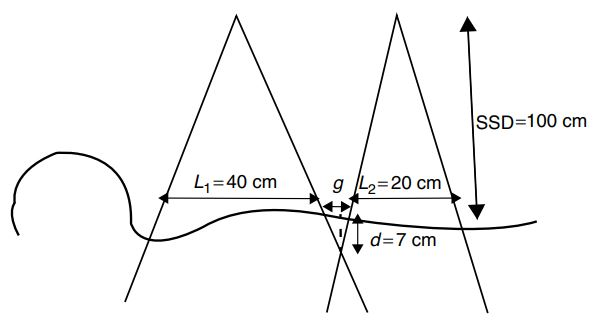
\includegraphics[width=0.5\textwidth]{Imagens/gapNeuroEixo.JPG}
            \end{center}
        
        \item No neuroeixo, são utilizados campos para tratar o crânio e campos para tratar a coluna. Caso os campos do crânio sejam não divergentes (utilizando a técnica de tenham meio campo bloqueado), então o colimador deverá girar em uma angulação que seja suficiente para ocorrer uma coincidencia geométrica entre o campo do crânio e o campo da coluna. Caso o feixe do crânio seja divergente, então além da angulação do colimador, também será necessário uma angulação da mesa em direção ao gantry para coincidir as divergências do feixe. 
        
        \item A figura abaixo representa o esquema para definição do ângulo de rotação do colimanor necessário para coincidir as divergências dos feixes:
        
            \begin{center}
                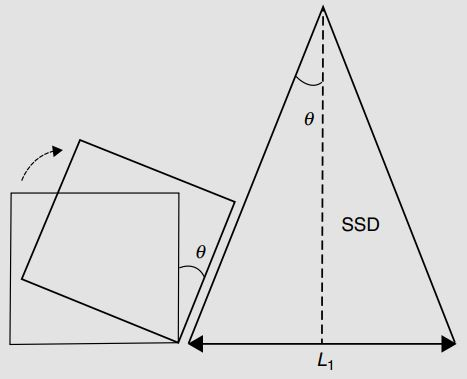
\includegraphics[width=0.5\textwidth]{Imagens/divergenciaColimador.JPG}
            \end{center}
        
        \item A figura abaixo representa o esquema para definição do ângulo de rotação da mesa  necessário para coincidir as divergências dos feixes do crânio com a coluna:
        
            \begin{center}
                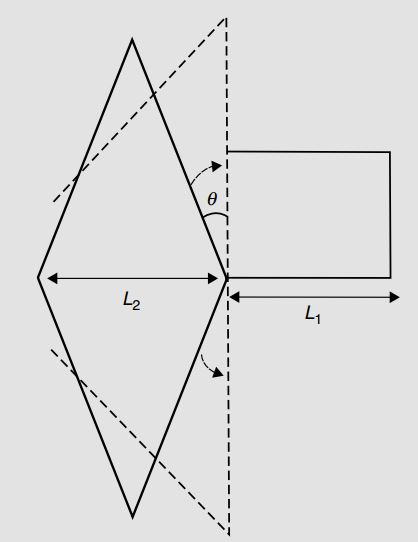
\includegraphics[width=0.5\textwidth]{Imagens/divergenciaMesa.JPG}
            \end{center}

        \item Um feixe de fótons de 10 MV, ao atravessar uma distância no pulmão, há um aumento na dose além do decido pulmonar de aproximadamente 2\% por cm de pulmão atravessado.
        
        \item Em um tratamento de mama com tangentes, não é recomendado utilizar filtros físicos na tangente interna caso seja desejável diminuir a dose espalhada na mama contralateral. 
        
        \item A técnica de tangente ampla é utilizada em tratamentos de mama que incluem a mamária interna, onde a tangente interna é definida de modo que a borda do campo é aberta no sentido da mama contralateral para englobar a mamária interna, enquanto a tangente externa abrange todo o tecido mamario. Porém, caso a configuração dos campos englobe muito tecido pulmonar, o recomendado é utilizar um campo separado de elétrons que case com as tangentes para reduzir a dose no pulmão. 
        
        \item Segundo o ICRU O GTV (Gross tumor volume) é o tumor visível em uma imagem e examinação física; O CTV (clinical target volume) é a região com risco de disseminação subclínica (microscópica); O ITV (integrated target volume) adiciona margens para considerar movimentaçõos conhecidas do tumor, devido à respiração por exemplo; O PTV (planning target volume) adiciona margens para considerar os erros aleatórios no setup do paciente. Portanto em ordem de tamanho do menor volume para o maior temos: $GTV < CTV < ITV < PTV$.
        
        \item O Volume tratado (Treated Volume - TV) é o volume coberto com a isodose de prescrição. O volume irradiado (Irradiated Volume - IV) é o volume coberto por 50\% da  isodose de prescrição

        \item De acordo com o ICRU a precisão da entrega da dose deve estar dentre $\pm 5\%$ do esperado. 

        \item A técnica do Four-Field Box (4 campos) é uma técnica de planejamento de tratamento onde quatro campo espaçados por uma angulação de \ang{90} entre si, contendo um campo anterior, um campo posterior, um campo lateral direito e um campo lateral esquedo que formam uyma distribuição de dose com formato quadrado ou retangular semelhante a uma caixa; Estes camos eram tipicamente utilizados para tratamentos de próstata antes da vinda do IMRT. 
        
        \item Para ocorrer um match entre campos adjacentes de fótons, o método mais típico é utilizando campos meio-bloqueados e realizar o match no isocentro onde não haverá divergência do feixe. Outra forma é combinando as divergências dos campos adjascentes angulando os campos um em relação ao outro, podendo utilizar angulações de mesa, colimador e gantry. 
            
        \item Os principais algoritmos de cálculo de dose utilizados em sistemas de planejamento são o pencil beam, superposition convolution e Monte Carlo. O algoritmo pencil beam tem sido largamente eliminado devido a incapacidade de considerar com precisão as heterogeneidades do meio como o pulmão e outros tecidos moles.
        
        \item Em planejamentos 3D, ao tratar um alvo central, pode ser uma maneira mais simplista utilizar campos AP/PA, porém esta geometria irá irradiar a medula tanto quanto o alvo. Para reduzir a dose na medula, normalmente é adicionado um campo obliquo evitando a medula ``off cord''; O campo AP/PA é utilizado para tratar em torno de 40 Gy (até um pouco abaixo da tolerância da medula) e então o campo obliquo evitando a medula é utilizado para complementar a dose. 
        
        \item Em um tratamento com geometria AP/PA para tratar a medula, como a medula fica mais posterior, o peso do campo posterior que está mais próximo a medula é definido entre 60\% a 70\%.
        
        \item Em um tratamento com par de filtros, os filtros são planejados para que eles fiquem com sua parte mais grossa juntas. O par de filtros é utilizado para reduzir a dose onde há o maior overlap entre os dois campos na menor profundidade.
        
        \item Em um tratamento de mama, as posições típicas para as bordas do campo são:
        
            \begin{itemize}[label=\textopenbullet]
                \item Borda Superior - Definida 1 cm acima do tecido mamário no qual é normalmente logo abaixo da cabeça clavicular;
                \item  Borda Inferior - É definida a 2 cm abaixo da linha inframamária;
                \item  Borda Medial - É definida na linha média do tórax ou no meio do esterno;
                \item Borda Lateral - É definida na linha axilar média. 
            \end{itemize}
        
        \item A densidade do Cerrobend é cerca de 83\% da densidade do chumbo; O Cerrobend é composto de 50\% de bismuto, 26.7\% de chumbo 13.3\% de estanho e 10\% de cádmio. 
        
        \item Cerrobend pode ser dimensionado para atenuar qualquer quantidade de um feixe, dependendo de sua espessura. Tipicamente, o bloco de Cerrobend é feito de modo que permita a transmissão de 5\% ou menos. Para isto é necessário aproximadamente 4.3 HVL's.
        
        \item Os blocos de cerrobend são focados na direção da fonte de raios-x cortando-os de modo que correspondam à divergência do feixe. Quando os blocos são cortados, um molde de isopor é colocado em uma bandeja acima de um filme radiográfico ou uma DRR. Uma caneta presa a um fio aquecido fixado em um ponto distante do isopor igual à distancia da fonte ao bloco, é utilizada para traçar o contorno da forma planejada para o bloco de acordo com o filme abaixo. O fio aquecido é inclinado para coincidir com a divergência do feixe originário de uma fonte a essa distância enquanto corta o isobor. O isopor cortado é então utilizado como molde para despejar o cerrobend. 

        \item Os MLC são feitos de tungstênio e diferentemente dos blocos de cerrobend, os MLC's são focados apenas na direção perpendicular à direção de movimentação do MLC, e não são focados na direção paralela ao movimento do MLC. A penumbra na direção paralela ao movimento do MLC é maior quando comparada aos blocos moldados de cerrobend. Os MLC' possuem lâminas de bordas arredondadas para minimizar a transmissão parcial na borda da lâmina. Os blocos de Cerrobend também ficam mais perto do paciente que o MLC, reduzindo ainda mais a penumbra. 
        
        \item A transmissão do MLC pode variar dependendo do fabricante. Os valores tipos para a transmissão atraves do MLC é de aproximadamente 2\% a 4\% para a transmissão interlâmina (entre as lâminas); 1\% a 2\% para a transmissão intra-lâmina (através da lâmina) e de 15\% a 24\% para a transmissão nas bordas das lâminas. A transmissão interlâminas incluem o uso de arranjos steps in groove entre as lâminas (``degrau e ranhura''). A figura abaixo mostra exemplos de MLC com esse arranjo para diferentes fabricantes. 
        
            \begin{center}
                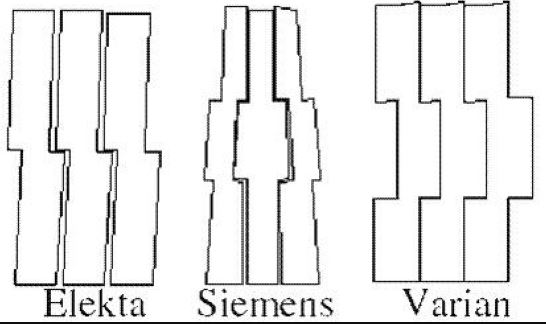
\includegraphics[width=0.5\textwidth]{Imagens/tongueInGroove.JPG}
            \end{center}
        
        \item Embora o feixe possa ser blindado com um bloco, ainda existirá dose na região abaixo ao bloco. Essa dose se deve a duas contribuições: A dose transmitida através do bloco e a dose espalhada pela região fora da região bloqueada. A dose embaixo do bloco é da ordem de 10\% da dose na região não bloqueada, dependendo da largura do bloco, pois um bloco mais estreito iria permitir mais espalhamento embaixo dele.


        \item Em tratamentos usando campos paralelos opostos com a dose prescrita no plano médio, a profundidade contendo a maior dose será na profundidade de dose máxima para essa geometria de campos. Para melhorar a uniformidade do plano, é ideal utilizar a maior energia de fótons disponível, pois quanto maior a energia, mais profunda é a penetração do feixe resultando em uma distribuição de dose mais uniforme. 
        
        \item Em campos filtrados, o ``hingle angle'' (ângulo da dobradiça) é a angulação entre os eixos centrais de dois campos filtrados. A figura abaixo mostra a definição do angulo hinge. 
        
            \begin{center}
                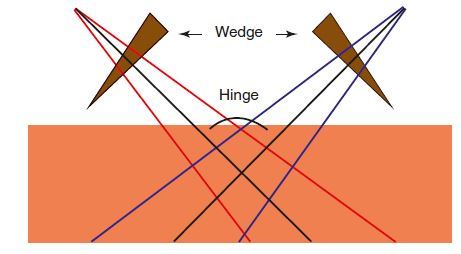
\includegraphics[width=0.5\textwidth]{Imagens/hinge.JPG}
            \end{center}
        
        \item Uma possibilidade de tratamento na pelve para tratamento de cancer retal é utilizadno a geometria de três campos compostos por dois campos laterais e um campo posterior, onde filtros podem ser utilizados para compensar a espessura diferencial do paciente a partir da região anterior para a posterior. Neste caso são utilizados filtros nos campos laterais, com a maior espessura do filtro no sentido posterior do paciente, apontando para a região do sacro pois esta região costuma ser mais fina que a região anterior. Outra vantagem de utilizar os filtros nessa posição é que permite reduzir os pontos quentes causados pela combinação dos campos laterais com o campo posterior.
        
        \item Em tratamentos de esôfago, normalmente é prescrita uma dose de 50,4 Gy. As possibilidades simples de tratamento são utilizando campos paralelos opostos AP/PA ou a técnica de 4 campos. A maior desvantagem em utilizar os campos paralelos opostos, é que a medula irá receber aproximadamente a dose prescrita ou até mesmo doses superiores pois os pontos quentes utilizando essa geometria estão mais perto da superficie do paciente. Este problema pode ser minimizado utilizando a geometria de 4 campos, porém sua maior desvantagem é que esta técnica resultará em uma maior dose nos pulmões. 
        
        \item A medida que o tamanho de campo aumenta, haverá uma maior contaminação de elétrons no feixe devido às interações de espalhamento com o colimador e com o ar, portanto haverá um aumento na dose na superfície. 

        \item As bandejas são utilizadas para segurar os blocos e são fontes de contaminação com elétrons. A medida que a bandeja de aproxima da superfície há uma menor oportunidade para os eletrons produzidos na bandeja se espalharem para fora da área do feixe e portanto aumenta a dose na superfície.
        
        \item Ao utilizar um feixe obliquo, a dose na superficie ira aumentar e a profundidade de dose máxima irá diminuir, quando comparada a um feixe com incidencia perpendicular. O maior aumento na dose superficial se dá para campos tangentes onde a dose na superfície é aproximadamente 4 vezes maior que a dose na superficie causada por um campo perpendicular. O feixe que incide perpendicularmente percorre uma profundidade maior até alcancar a profundidade de dose máxima definida para um feixe perpendicular, portanto a profundidade de dose máxima irá ocorrer em uma profundidade perpendiculas mais próxima à superfície. 

        \item A ùnica forma de aumentar a dose na superfície sem diminuir a profundidade de penetração é utilizando um ``Beam Spoiler''. O Beam spoiler consiste em uma bandeja de plástico colocada na frente do feixe, próximo à superfície da pele. O Beam spoiler aumenta a contaminação do feixe com elétrons superficializando a dose, ao mesmo tempo que não atenua o feixe significativamente mantendo a mesma penetração.
        
        \item A maior diferença entre um bolus e um filtro compensador, é que o bolus possui uma espessura uniforme e seu objetivo é superficializar a dose na pele do paciente. Já os compensadores tem como objetivo compensar os contornos irregulares da superfície do paciente. Os compensadores são então producidos especificamente para cada paciente. Um filtro é considerado um tipo de compensador que compensa as variações no tecido em apenas uma direção, não sendo customizados para cada paciente. 
    \end{itemize}
\end{exemplo}


\bibliography{ref.bib}
\end{document}